\documentclass[a4paper,10pt]{jsarticle}
\usepackage{memo1}
% - - - - - - - - - 以下,個別編集箇所 - - - - - - - - - 
%タイトル
%左上のヘッダーにも表示される
\title{非平衡多体理論}
%署名
\affiliation{中国科学院大学 Kavli理論科学研究所}
\author{藤本純治}
%メールアドレス
\email{junji@ucas.ac.cn}
%作成・更新日とバージョンを書けばいいと思うよ
\date{2020-04-05〜}
%
\graphicspath{{./figure/}}
% - - - - - - - - - 以上,個別編集箇所 - - - - - - - - - 
\usepackage{memo2}
\usepackage{macro}
%\usepackage{diff}
%
\newcommand{\mH}{\mathrm{H}}
\newcommand{\kF}{k_{\mathrm{F}}}
%
% 以下2つは参考文献の書式を指定する.bibtex を使わない場合はコメントアウト
%\bibliographystyle{apsrev4-1}
%\usepackage[numbers]{natbib}
%
\begin{document}
%
\maketitle

% abstract is here.
\begin{abstract}
このメモは主に,H.~J.~W.~HaugとA.-P.~Jauhoによる著書"\textit{Quantum Kinetics in Transport and Optics of Semiconductors}"のPart IIに従う.
まず前準備として,径路順序Green関数を定義し,それがcausal, greater, lesser, antitime-ordered Green関数に分解できることを見る.
次に,径路順序Green関数の摂動展開について調べる.
それから,径路順序Green関数の積を実時間の各種Green関数の積に書き換えるときに有用なLangreth則を紹介する.
以上の準備ののち,lesser Green関数の時間発展を記す方程式である量子運動学的方程式をKadanoff-Baym形式とKeldysh形式で議論する.
そしてWiegner表示を導入し,勾配展開することで量子運動学的方程式がBoltzmann方程式を再現することを見る.
また,この再現においてスペクトル関数が十分に絞られていることが必要であることを確認する.
\end{abstract}

\setcounter{section}{3}

%-%-%-%-%-%-%-%-%-%--%-%-%-%-%-%-%-%-%-%
\section{径路順序Green関数}
%-%-%-%-%-%-%-%-%-%--%-%-%-%-%-%-%-%-%-%
%-%-%-%-%-%-%-%-%-%-
\subsection{\label{sec:4.1}総説}
%-%-%-%-%-%-%-%-%-%-
非平衡問題は以下のように定式化される.
以下のハミルトニアンのもとで時間発展する系を考える.
\begin{align}
H
	& = h + H' (t)
.\end{align}
ここでハミルトニアンにおいて時間に依存しない部分$h$を2つの部分に分ける:$h = H_0 + H_i$,ただし$H_0$は(対角化でき,それゆえにWickの定理が適用できるという意味で)``シンプル''であり,$H_i$は(問題の多体的側面を含んでおり,それゆえに特別な取り扱いが必要であるという意味で)``複雑''であるとする.
さらに仮定として,非平衡部分は$t < t_0$においては消えるとする.

適切な時点で$t_0 \to - \infty$と置き換えることがしばしばある.
この手続きは問題の取り扱いを単純化し,非平衡理論の構造を可能な限り簡潔に示すことができるので,まず初めはこの極限を採用する.
しかし,そのような極限をとってしまうと過渡現象(transient phenomena)を取り扱うことが不可能になってしまう.
過渡現象は我々が述べたい中心的話題の一つなので,また必要なときにこの点に戻ってくることにする.
(このメモでは戻ってきません.)

摂動を加える前では,系は熱平衡の密度行列
\begin{align}
\rho (h)
	& = \frac{ \exp( - \beta h) }{ \mathrm{Tr}[ \exp(- \beta h) ] }
\end{align}
によって記述されている.
$\beta = 1 / \kB T$は逆温度である.
遂行すべきことは,与えられた観測量の期待値を計算することである.
その観測量に関連づけられた量子力学的な演算子を$O$とすると,時刻$t > t_0$においては,その期待値は
\begin{align}
\langle O (t) \rangle
	& = \mathrm{Tr} [ \rho (h) O_{H} (t) ]
\label{def:O}
\end{align}
と書ける.
下付き添字$H$は,Heisenberg描像で,その時間依存性は全ハミルトニアン$H$によって支配されていることを意味している.
定義~(\ref{def:O})は,容易に2時刻(あるいはそれ以上)の量(たとえばGreen関数や相関関数)に一般化することができる.

ここで,式~(\ref{def:O})において,何らかの時間依存した密度行列ではなく,熱平衡密度行列を用いたことを記しておく.
これは,物理的には,$h$に含まれている熱力学的な自由度は,$H'(t)$に含まれる速い振動に即座に追従しないことを意味している.
この他に選び方があってもよいが,それに伴う困難~\footnote{たとえば,文献~\cite{Mahan}のp.214-216を参照.}を避けるため,ここではこの選び方を採用する.
潜在的にとても見込みのある代替的方法は,期待値に含まれる熱平衡密度行列を,ある適切な一般化したものに置き換えることで構成され,それはHershfieldなどによって指摘され~\cite{Hershfield},近年いくつかの文献~\cite{Bokes,Coleman,Doyon,Han}において精巧化された.
この方法の可能性についても,半導体微細構造における時間依存輸送について書かれた13章で述べる.

%-%-%-%-%-%-%-%-%-%-
\subsection{\label{sec:4.2}2つの変換}
%-%-%-%-%-%-%-%-%-%-
式~(\ref{def:O})を攻略する一般的な戦略は,熱平衡の場合に似ている.
すなわち,$O_H (t)$の``望みが薄そうなほどに複雑な"時間依存性を,より簡単な$O_{H_0}$の時間依存の形へと変換させることである.
消去すべき演算子は2つある;時間依存する外的摂動$H' (t)$と``複雑な''相互作用項$H_i$である.
したがって,熱平衡の場合よりも込み入った変換を行うことが予想される.
しかしながら,適当に一般化することにともなって,非平衡と熱平衡の定式化を構造的に等価に行うことができると示せる.

最初に,$O_H$の時間依存性を$O_h$の時間依存性に書き換える.
これは,次の関係式を用いて行う.
\begin{align}
O_H (t)
	& = v_h^{\dagger} (t, t_0) O_h (t) v_h (t, t_0)
\label{eq:O_H}
,\end{align}
ここで
\begin{align}
v_h (t, t_0)
	& = \mathrm{T} \left\{ \exp \left[ - \zi \int_{t_0}^{t} \dd{t'} H'_h (t') \right] \right\}
,\end{align}
また$H'_h (t)$は$H' (t)$の相互作用表示で,
\begin{align}
H'_h (t)
	& = e^{\zi h (t - t_0)} H' (t) e^{- \zi h (t - t_0)}
\end{align}
で与えられ,$\mathrm{T}$は遅い時刻を左から並べていく時間順序演算子を表す.

ここで径路順序量を導入しよう.
表式~(\ref{eq:O_H})はまた別の,しかし等価な表式に書き換えることができる.
\begin{align}
O_H (t)
	& = \mathrm{T}_{C_t} \left\{ \exp \left[ - \zi \int_{C_t} \dd{\tau} H'_h (\tau) \right] O_h (t) \right\}
\label{eq:O_H_Ct}
,\end{align}
ただし,径路$C_t$は図~\ref{fig:4.1}に示す.
%%%%%%%%%%%%%%%%%%%%%%%%%%%%%%%%%%%%%%%%%%
\begin{figure}[thbp]
\centering
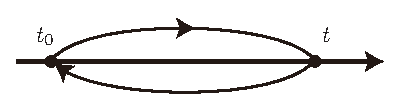
\includegraphics[width=0.5\linewidth]{4.1.eps}
\caption{\label{fig:4.1}径路$C_t$.}
\end{figure}
%%%%%%%%%%%%%%%%%%%%%%%%%%%%%%%%%%%%%%%%%%
以下では,複素径路上の時刻を表す変数をギリシャ文字で表記し,実時刻を表す変数に対してはローマ文字を用いるようにする.
径路$C_t$は,$t_0$から$t$に向けて実軸上を走り,もう一度$t$から$t_0$に戻る.
(あるいは,実軸の少しだけ上を走る;$H' (t)$が解析的に連続であるならば何ら問題は起こらない.)
径路順序演算子$T_{C_t}$の意味は,次のようになる.
$t_1$と$t_2$が$C_t$上の2つの時刻を表すとして,径路上で$t_2$が$t_1$に対して後に現れるならば,$T_{C_t} \{H'_h (t_1) H'_h (t_2)\} = H'_h (t_2) H'_h (t_1)$のように,後ろの時刻を左に並べかえる演算を表す.
次の計算で径路上に定義された関数の性質を示す.

%-%-%-%-%-%-%-%-%-%-%-
\textbf{式~(\ref{eq:O_H})と式~(\ref{eq:O_H_Ct})が等しいことを示す}\\
%-%-%-%-%-%-%-%-%-%-%-
径路上で定義された関数について理解を深めるために,ここで式~(\ref{eq:O_H})と式~(\ref{eq:O_H_Ct})が厳密に等しいことを示そう.
まず,式~(\ref{eq:O_H_Ct})に対して$\exp$を展開する.
\begin{align}
\mathrm{T}_{C_t} \left\{ \exp \left[ - \zi \int_{C_t} \dd{\tau} H'_h (\tau) \right] O_h (t) \right\}
	& = \sum_{n = 0}^{\infty} \frac{(-\zi)^n}{n!} \int_{C_t} \dd{\tau_1} \cdots \int_{C_t} \dd{\tau_n}
		\mathrm{T}_{C_t} \left[
			H'_h (\tau_1) \cdots H'_h (\tau_n) O_h (t)
		\right]
\label{eq:4.8}
.\end{align}
ここで,径路$C_t$を2つに分ける:
\begin{align}
\int_{C_t}
	& = \int_{\rightarrow} + \int_{\leftarrow}
,\end{align}
ただし$\int_{\rightarrow}$は$t_0$から$t$へ向かい,$\int_{\leftarrow}$は$t$から$t_0$に戻ることを表している.
よって,式~(\ref{eq:4.8})の$n$次の項は$2^n$個の項に分けられるが,そのうちの1つについて考えてみると,
\begin{align}
& \int_{\rightarrow} \dd{\tau_1} \int_{\rightarrow} \dd{\tau_2} \int_{\leftarrow} \dd{\tau_3} \cdots \int_{\leftarrow} \dd{\tau_n}
	\mathrm{T}_{C_t} \left[ H'_h (\tau_1) \cdots H'_h (\tau_n) O_h (t) \right]
\notag \\ & \hspace{1em}
	= \int_{\leftarrow} \dd{\tau_3} \cdots \int_{\leftarrow} \dd{\tau_n} \mathrm{T}_{\leftarrow} \left[ H'_h (\tau_3) \cdots H'_h (\tau_n) \right]
	O_h (t)
	\int_{\rightarrow} \dd{\tau_1} \int_{\rightarrow} \dd{\tau_2} \mathrm{T}_{\rightarrow} \left[ H'_h (\tau_1) H'_h (\tau_2) \right]
.\end{align}
$2^n$個の項のうち,$m \,(m = 0, \cdots, n)$個の$\int_{\rightarrow}$を含み,$n-m$個の$\int_{\leftarrow}$を含む項は$n! / [m! (n-m)!]$つあり,それらは全て等しく寄与する.
よって,
\begin{align}
& \int_{C_t} \dd{\tau_1} \cdots \int_{C_t} \dd{\tau_n} \mathrm{T}_{C_t} \left[ H'_h (\tau_1) \cdots H'_h (\tau_n) O_h (t) \right]
\notag \\ & \hspace{1em}
	= \sum_{m = 0}^{n} \frac{n!}{m! (n-m)!}
	\int_{\leftarrow} \dd{\tau_{m+1}} \cdots \int_{\leftarrow} \dd{\tau_n} \mathrm{T}_{\leftarrow} \left[ H'_h (\tau_{m+1}) \cdots H'_h (\tau_n) \right]
	O_h (t)
\notag \\ & \hspace{4em} \times
	\int_{\rightarrow} \dd{\tau_1} \cdots \int_{\rightarrow} \dd{\tau_m} \mathrm{T}_{\rightarrow} \left[ H'_h (\tau_1) \cdots H'_h (\tau_m) \right]	
\label{eq:4.11}
\end{align}
と書ける.
$k = n - m$と変数を書き換え,Kroneckerのデルタを用いて$k + m = n$を保ちつつ$k$と$m$の和を$0$から$\infty$までとるように書き換える.
すると,式~(\label{eq:4.11})は,
\begin{align}
& \to \sum_{m, k = 0}^{\infty} \frac{n!}{m! k!} \delta_{n, k + m}
	\left\{
		\int_{\leftarrow} \dd{\tau_1} \cdots \int_{\leftarrow} \dd{\tau_k} \mathrm{T}_{\leftarrow} \left[ H'_h (\tau_1) \cdots H'_h (\tau_k) \right]
	\right\}
	O_h (t)
\notag \\ & \hspace{3em} \times
	\left\{
		\int_{\rightarrow} \dd{\tau_1} \cdots \int_{\rightarrow} \dd{\tau_m} \mathrm{T}_{\rightarrow} \left[ H'_h (\tau_1) \cdots H'_h (\tau_m) \right]
	\right\}
.\end{align}
さて,式~(\ref{eq:4.8})に戻ると,$n$の和は$\delta_{n, k+m}$のために簡単に実行でき,以下を得る.
\begin{align}
& \mathrm{T}_{C_t} \left\{ \exp \left[ - \zi \int_{C_t} \dd{\tau} H'_h (\tau) \right] O_h (t) \right\}
\notag \\ & \hspace{1em}
	= \sum_{k = 0}^{\infty} \frac{(-\zi)^k}{k!}
	\left\{
		\int_{\leftarrow} \dd{\tau_1} \cdots \int_{\leftarrow} \dd{\tau_k} \mathrm{T}_{\leftarrow} \left[ H'_h (\tau_1) \cdots H'_h (\tau_k) \right]
	\right\}
	O_h (t)
\notag \\ & \hspace{3em} \times
	\sum_{m = 0}^{\infty} \frac{(-\zi)^m}{m!}
	\left\{
		\int_{\rightarrow} \dd{\tau_1} \cdots \int_{\rightarrow} \dd{\tau_m} \mathrm{T}_{\rightarrow} \left[ H'_h (\tau_1) \cdots H'_h (\tau_m) \right]
	\right\}
.\end{align}
しかして,$O (t)$に左右から掛けられている因子を見比べると,それらがそれぞれ$v_h^{\dagger} (t_0, t)$と$v_h (t_0, t)$に等しいことが分かる.
以上で,式~(\ref{eq:O_H})と式~(\ref{eq:O_H_Ct})の等価性が示された.
■

径路順序演算子は,熱平衡理論と全く同じように非平衡理論を構築するのに強力な形式的道具である.

さて,径路順序Green関数(contour-ordered Green function)を定義しよう:
\begin{align}
G (x, x')
	& \equiv - \zi \langle \mathrm{T}_C [ \psi^{}_{\mH} (x) \psi^{\dagger}_{\mH} (x') ] \rangle
\label{def:G}
,\end{align}
ただし,径路$C$は$t_0$に始まり,同じ$t_0$で終わる図~\ref{fig:4.2}のような,実軸に沿って$t$と$t'$を一度だけ通るような径路を表す.
ここで,Part Iと同じように,$\psi_{\mH} (x)$はフェルミオンの場の演算子で,Heisenberg表示を表す.
また,以下では$x = (\br, t)$あるいは$x = (\br, \tau)$という簡略表記を用いる\footnote{原文では$1 = (\bm{x}_1, t_1$などと書かれているが,個人的にはあまり馴染みがないため,馴染みのある表記に書き換えた.}.
%%%%%%%%%%%%%%%%%%%%%%%%%%%%%%%%%%%%%%%%%%
\begin{figure}[thbp]
\centering
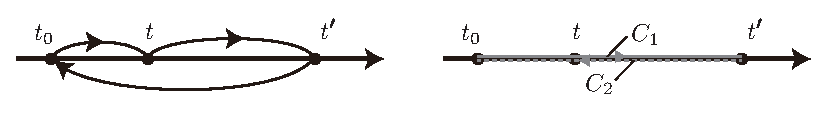
\includegraphics[width=\linewidth]{4.2.eps}
\caption{\label{fig:4.2}径路$C$.}
\end{figure}
%%%%%%%%%%%%%%%%%%%%%%%%%%%%%%%%%%%%%%%%%%

非平衡の理論において径路順序Green関数は,熱平衡の理論における因果Green関数に類似の役割を果たす.
すなわち,以下で見るように,Wickの定理に基づいた摂動展開を有している.
しかしながら,時刻ラベル$\tau$と$\tau'$は径路上の2つの分枝にあるため,それらがどの分枝にあるのかが問題になる.
$\tau$と$\tau'$は,図~\ref{fig:4.2}の径路の2つの分枝のどちらの分枝にもありうるので,4つの可能性がある.
ゆえに,式~(\ref{def:G})は,4つの異なる関数を内包する.
\begin{align}
G (x, x')
	& = \left\{
	\begin{array}{l l}
		G_{\mathrm{c}} (x, x')
	&	t, t' \in C_1
	\\	G^{>} (x, x')
	&	t \in C_2, t' \in C_1
	\\	G^{<} (x, x')
	&	t \in C_1, t' \in C_2
	\\	G_{\tilde{\mathrm{c}}} (x, x')
	&	t, t' \in C_2
	.\end{array}
	\right.
\end{align}
ここで,因果 (あるいは時間順序) Green関数$G_{\mathrm{c}}$を
\begin{align}
G_{\mathrm{c}} (x, x')
	& = - \zi \langle \mathrm{T} [ \psi^{}_{\mH} (x) \psi^{\dagger}_{\mH} (x') ] \rangle
\notag \\
	& = - \zi \theta (t - t') \langle \psi^{}_{\mH} (x) \psi^{\dagger}_{\mH} (x') \rangle
		+ \zi \theta (t' - t) \langle \psi^{\dagger}_{\mH} (x') \psi^{}_{\mH} (x) \rangle
\label{def:G_c}
\end{align}
のように,また``greater'' Green関数$G^{>}$を
\begin{align}
G^{>} (x, x')
	& = - \zi \langle \psi^{}_{\mH} (x) \psi^{\dagger}_{\mH} (x') \rangle
\label{def:G_greater}
\end{align}
のように,そして``lesser'' Green関数$G^{<}$を
\begin{align}
G^{<} (x, x')
	& = + \zi \langle \psi^{\dagger}_{\mH} (x') \psi^{}_{\mH} (x) \rangle
\label{def:G_lesser}
\end{align}
のように,最後に反時間順序Green関数$G_{\tilde{\mathrm{c}}}$を
\begin{align}
G_{\tilde{\mathrm{c}}} (x, x')
	& = - \zi \langle \tilde{\mathrm{T}} [ \psi^{}_{\mH} (x) \psi^{\dagger}_{\mH} (x') ] \rangle
\notag \\
	& = - \zi \theta (t' - t) \langle \psi^{}_{\mH} (x) \psi^{\dagger}_{\mH} (x') \rangle
		+ \zi \theta (t - t') \langle \psi^{\dagger}_{\mH} (x') \psi^{}_{\mH} (x) \rangle
\label{def:G_antitime-ordered}
\end{align}
のように導入した.
$G_{\mathrm{c}} + G_{\tilde{\mathrm{c}}} = - \zi \langle \psi^{}_{\mH} (x) \psi^{\dagger}_{\mH} (x') \rangle + \zi \langle \psi^{\dagger}_{\mH} (x') \psi^{}_{\mH} (x) \rangle = G^{>} + G^{<}$なので,独立な関数は3つである.
この自由度の選び方には幾つかの流儀があり,幾つもの表記法が見られる.
我々の目的のために最も最適な関数は$G^{>}$と$G^{<}$(これらはしばしば「相関関数」という一般的な名前で書かれることもある)と,先進Green関数と遅延Green関数である.
先進Green関数は
\begin{align}
G^{\A} (x, x')
	& = \zi \theta (t' - t) \langle \{ \psi^{}_{\mH} (x), \psi^{\dagger}_{\mH} (x') \} \rangle
\notag \\
	& = - \theta (t' - t) \left[ G^{>} (x, x') - G^{<} (x, x') \right]
\label{def:G^A}
\end{align}
と遅延Green関数は
\begin{align}
G^{\R} (x, x')
	& = - \zi \theta (t - t') \langle \{ \psi^{}_{\mH} (x), \psi^{\dagger}_{\mH} (x') \} \rangle
\notag \\
	& = \theta (t - t') \left[ G^{>} (x, x') - G^{<} (x, x') \right]
\label{def:G^R}
\end{align}
で定義される.
ここで$\{A, B\} = A B + B A$は反交換関係を表す.
$G^{\R} (x, x') - G^{\A} (x, x') = G^{>} (x, x') - G^{<} (x, x')$が見てとれる.
後ろの章にて,$G^{>}, G^{<}, G^{\R}, G^{\A}$の物理的な解釈について詳細に議論する予定である({\color{red}どこ?}).

必要な関数の定義を終えて,本節の中心課題に戻るとする.
すなわち,径路順序Green関数~(\ref{def:G})をWickの定理を用いられる形に変形するということだ.
第一段階として,式~(\ref{eq:O_H_Ct})を導いた解析,つまり$H$依存性を$h$依存性に書き換えることをここでも繰り返す.
その結果は,\footnote{{\color{red} このあたりの計算が端折られている点が,あまり親切ではないと感じる点ではある.}}
\begin{align}
G (x, x')
	& = - \zi \langle \mathrm{T}_C [ S_{C}^{H} \psi^{}_{h} (x) \psi^{\dagger}_{h} (x') ] \rangle
\label{eq:G_H}
,\end{align}
ここで,$\psi^{(\dagger)}_{h} (x) = e^{\zi h (t - t_0)} \psi^{(\dagger)} (\br) e^{- \zi h (t - t_0)}$は$\psi^{(\dagger)} (\br)$の相互作用表示であり,
\begin{align}
S_{C}^{H}
	& = \exp \left[ - \zi \int_{C} \dd{\tau} H'_{h} (\tau) \right]
\end{align}
である.
ダイヤグラム的摂動理論が存在することを示すためには,さらにもう一段階の式変形が必要である.
$h = H_0 + H_i$のように$h$が2つの項を含んでいたこと,そしてWickの定理が$H_0$に対してのみ機能することを思い出せば,$h$依存性を$H_0$依存性に置き換えなければならないことになる.
また,密度行列にも$h$が含まれており,それゆえに,式~(\ref{eq:G_H})には,$\rho (h)$, $S_{C}^{H}$, $\psi^{}_h (x)$, $\psi^{\dagger}_h (x')$の合計で4箇所に$h$が含まれていることに留意する.

この式変形は,いくぶん退屈であるが躓くところはほとんどないはずなので,詳細は文献~\cite{RammerRMP}に譲り,最終結果を記すだけで十分だろう.~\footnote{{\color{red} このあたりの計算が端折られている点が,あまり親切ではないと感じる点ではある.}}
\begin{align}
G (x, x')
	& = - \zi \frac{ \mathrm{Tr} \left\{ \mathrm{T}_{C_v} [ S_{C_v}^i S'_{C} \psi^{}_{H_0} (x) \psi^{\dagger}_{H_0} (x') ] \right\} }%
		{ \mathrm{Tr} [ \rho_0 \mathrm{T}_{C_v} ( S_{C_v}^i S'_{C} ) ] }
\label{eq:G_H0}
,\end{align}
ここで,密度行列$\rho_0$は
\begin{align}
\rho_0
	& = \frac{\exp (- \beta H_0)}{\mathrm{Tr} [ \exp (- \beta H_0) ]}
\end{align}
で与えられ,
\begin{align}
S'_{C}
	& = \exp \left[ - \zi \int_{C} \dd{\tau} H'_{H_0} (\tau) \right]
\notag
, \\
S_{C_v}^i
	& = \exp \left[ - \zi \int_{C_v} \dd{\tau} H_{i, H_0} (\tau) \right]
\end{align}
であるが,$H'_{H_0}$と$H_{i, H_0}$は$H_0$による時間発展を表す;
\begin{align*}
H'_{H_0} (t)
	= e^{\zi H_0 (t - t_0)} H' e^{- \zi H_0 (t - t_0)}
, \qquad
H_{i, H_0} (t)
	= e^{\zi H_0 (t - t_0)} H_i e^{- \zi H_0 (t - t_0)}
.\end{align*}
また,径路$C$は図~\ref{fig:4.2}にて定義したものであり,径路$C_v$は図~\ref{fig:4.3}に示した.
%%%%%%%%%%%%%%%%%%%%%%%%%%%%%%%%%%%%%%%%%%
\begin{figure}[thbp]
\centering
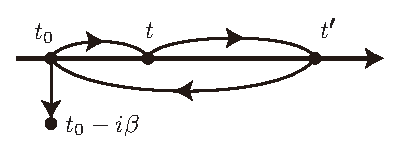
\includegraphics[width=0.5\linewidth]{4.3.eps}
\caption{\label{fig:4.3}径路$C_v$.}
\end{figure}
%%%%%%%%%%%%%%%%%%%%%%%%%%%%%%%%%%%%%%%%%%

式~(\ref{eq:G_H0})は,重要な結果であり,見た目の複雑さに関わらず,多くの魅力的な性質を有している.
まず第一に,厳密であるという点である.
次に,全ての時間依存性は,$H_0$によって記されているため,「解くことができる」.
特に,平方完成できる密度行列($\sim \exp( - \beta H_0)$)のために,Wickの定理を用いることが可能であり,そのためFeynmanダイヤグラムを非平衡系の問題に構成することができる.
ちょうど熱平衡系のときのように,分母が非連結のダイヤグラムからの寄与を打ち消してくれるのである.

以下のようにこの節の中心的な結果をまとめられる.
すなわち,熱平衡理論と非平衡理論は構造的に等価であり,それらの違いは,単に実時間における積分が径路上の積分に置き換えられただけである.


%-%-%-%-%-%-%-%-%-%-
\subsection{\label{sec:4.3}解析接続}
%-%-%-%-%-%-%-%-%-%-
式~(\ref{eq:G_H0})は強力な公式であるが,径路上の積分を実時間の積分に置き換えられなければ,実用的とは言い難い.
実時間積分への書き換えの手続きは解析接続と呼ばれ,多くの異なる定式化がこれまで行われてきた.
ここではLangreth~\cite{Langreth}によるKadanoffとBaymの方法~\cite{Kadanoff-Baym}を詳しく記す.

前節で示したように,径路順序Green関数は,熱平衡理論における時間順序Green関数と同じ摂動展開の構造を持っている.
その結果,自己エネルギー汎関数を定義することができて,熱平衡のときと同じようにDyson方程式を径路順序Green関数は有する:
\begin{align}
G (x, x')
	& = G_0 (x, x')
		+ \int \dd{\br_1} \int_{C_v} \dd{\tau_1} G_0 (x, x_1) U (x_1) G (x_1, x')
\notag \\ & \hspace{1em}
		+ \int \dd{\br_1} \int \dd{\br_2} \int_{C_v} \dd{\tau_1} \int_{C_v} \dd{\tau_2}
			G_0 (x, x_1) \varSigma (x_1, x_2) G (x_2, x')
\label{eq:Dyson}
,\end{align}
ここでハミルトニアンにおける非平衡を与える項は1体のポテンシャル$U$で表されることを仮定した.
そして相互作用は(既約な)自己エネルギー$\varSigma [G]$にすべて含まれている.

\ref{sec:4.1}~節で言及したが,$t_0 \to - \infty$とすることができるならば問題は簡略化する.
もし相互作用が断熱的に印加されたのならば,$[t_0, t_0 - \zi \beta]$区間からの寄与は消えるのである.
この手続きによる情報の欠落は初期相関に関係している.
多くの現実的な状況,たとえば定常輸送のような場合では,系が定常状態に達したとき初期相関は相互作用によって消失することは尤もらしい.
その一方で,過渡的な応答を調べようとしたとき,初期相関は重要になりえて,興味深い問題を提示しているが,研究者による注目はごく限られてものに留まっている~\cite{Yu,Wagner1991}.
また,ごく最近になって,径路の複素部分を数値的に計算するという重要な研究が行われた~\cite{Dahlen,Danielewicz1984a,Danielewicz1984b,vanLeeuwen}.
ともあれ,ここでは$t_0 \to - \infty$の極限をとろう.
この極限では径路$C_v$と$C$は一致し,結局は径路$C$のみを考えればよい.

%-%-%-%-%-%-%-%-%-%-%-
\textbf{Langrethの定理.}\\
%-%-%-%-%-%-%-%-%-%-%-
Dyson方程式~(\ref{eq:Dyson})を考えるうえで,$C = A B$,あるいは厳密に表現すると,
\begin{align}
C (t, t')
	& = \int_{C} \dd{\tau} A (t, \tau) B (\tau, t')
\label{eq:C=AB}
\end{align}
という構造と,同様の3つ以上の積を扱うことになる.
ここでは時間変数のみに関心があるので,その他の空間変数やスピンなどについては(明らかな行列構造を有するのみなので)省略することにする.
式~(\ref{eq:C=AB})を評価するために,まず$t$を径路$C$の前半部分($t_0 \to t'$の径路)にあるとし,また$t'$は径路$C$の後半部分($t' \to t_0$)にある場合を考えよう.
式~(\ref{def:G_c})〜(\ref{def:G^R})での議論によれば,lesser成分を解析することになる.

%%%%%%%%%%%%%%%%%%%%%%%%%%%%%%%%%%%%%%%%%%
\begin{figure}[thbp]
\centering
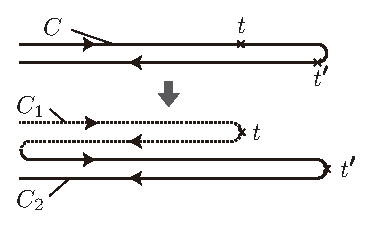
\includegraphics[width=0.5\linewidth]{4.4.eps}
\caption{\label{fig:4.4}径路$C$の変形.}
\end{figure}
%%%%%%%%%%%%%%%%%%%%%%%%%%%%%%%%%%%%%%%%%%
次の段階として図~\ref{fig:4.4}に示すように径路を変形させる.
その結果,式~(\ref{eq:C=AB})は以下のようになる.
\begin{align}
C^{<} (t, t')
	& = \int_{C_1} \dd{\tau} A (t, \tau) B^{<} (\tau, t')
		+ \int_{C_2} \dd{\tau} A^{<} (t, \tau) B (\tau, t')
\label{eq:4.29}
.\end{align}
ここで,第1項において$B$に$<$の記号が現れているが,径路の意味において積分変数$\tau$は常に$t'$より以前の時刻を表すという事実を用いた\footnote{※$A$や$B$を具体的に何と言及せずに記しているが,Green関数の他にも自己エネルギーもありえる.しかしここまでで自己エネルギーのlesser成分は未定義なので,あまり良い記述とは言えないように思う.}.
同様の論理で第2項にも記号$<$が付与されている.
さて,式~(\ref{eq:4.29})の第1項を考え,その積分を2つの部分に分けると,
\begin{align}
\int_{C_1} \dd{\tau} A (t, \tau) B^{<} (\tau, t')
	& = \int_{-\infty}^{t} \dd{t_1} A^{>} (t, t_1) B^{<} (t_1, t')
		+ \int_{t}^{-\infty} \dd{t_1} A^{<} (t, t_1) B^{<} (t_1, t')
\notag \\
	& = \int_{-\infty}^{\infty} \dd{t_1} \left[ \theta (t - t_1) \left( A^{>} (t, t_1) - A^{<} (t, t_1) \right) \right] B^{<} (t_1, t')
\notag \\
	& \equiv \int_{-\infty}^{\infty} \dd{t_1} A^{\R} (t, t_1) B^{<} (t_1, t')
,\end{align}
ただし,記号$>, <$をgreater, lesser関数~(\ref{def:G_greater})と(\ref{def:G_lesser})の意味合いで導入し,遅延関数の定義~(\ref{def:G^R})を拡張する形で記号$\R$を導入した.
第2項についても同様に,
\begin{align*}
\int_{C_2} \dd{\tau} A^{<} (t, \tau) B (\tau, t')
	& = \int_{-\infty}^{t'} \dd{t_1} A^{<} (t, t_1) B^{<} (t_1, t')
		+ \int_{t'}^{-\infty} \dd{t_1} A^{<} (t, t_1) B^{>} (t_1, t')
\\	& = \int_{-\infty}^{\infty} \dd{t_1} A^{<} (t, t_1) \left[ \theta (t' - t_1) \left( B^{<} (t_1, t') - B^{>} (t_1, t') \right) \right]
\\	& \equiv \int_{-\infty}^{\infty} \dd{t_1} A^{<} (t, t_1) B^{\A} (t_1, t')
,\end{align*}
ただし記号$\A$を先進関数~(\ref{def:G^A})を拡張する形で導入した.
これらをまとめると,第一のLangrethの結果を得る:
\begin{align}
C^{<} (t, t')
	& = \int_{-\infty}^{\infty} \dd{t_1} \left[ A^{\R} (t, t_1) B^{<} (t_1, t') + A^{<} (t, t_1) B^{\A} (t_1, t') \right]
\label{eq:C^<}
.\end{align}
また,$<$を$>$に置き換えるだけで,$>$成分について同様の結果が得られる.
実際,$t$が$t' \to t_0$の径路上にあり,$t'$が$t_0 \to t'$の経路上にある場合,
\begin{align*}
C^{>} (t, t')
	& = \int_{C'_1} \dd{\tau} A^{>} (t, \tau) B (\tau, t')
		+ \int_{C'_2} \dd{\tau} A (t, \tau) B^{>} (\tau, t')
\\	& = \int_{-\infty}^{t'} \dd{t_1} A^{>} (t, t_1) B^{<} (t_1, t')
		+ \int_{t'}^{-\infty} \dd{t_1} A^{>} (t, t_1) B^{>} (t_1, t')
\\	& \hspace{1em}
		+ \int_{-\infty}^{t} \dd{t_1} A^{>} (t, t_1) B^{>} (t_1, t')
		+ \int_{t}^{-\infty} \dd{t_1} A^{<} (t, t_1) B^{>} (t_1, t')
\\	& = \int_{-\infty}^{\infty} \dd{t_1} A^{>} (t, t_1) \left[ \theta (t' - t_1) \left( B^{<} (t_1, t') -  B^{>} (t_1, t') \right) \right]
\\	& \hspace{1em}
		+ \int_{-\infty}^{\infty} \dd{t_1} \left[ \theta (t - t_1) \left( A^{>} (t, t_1) - A^{<} (t, t_1) \right) \right] B^{>} (t_1, t')
\\	& = \int_{-\infty}^{\infty} \dd{t_1} \left[ A^{\R} (t, t_1) B^{>} (t_1, t') + A^{>} (t, t_1) B^{\A} (t_1, t') \right]
,\end{align*}
ただし$C'_1$, $C'_2$はそれぞれ$-\infty \to t' \to -\infty$と$-\infty \to t \to -\infty$の径路を表す.

この結果~(\ref{eq:C^<})は,3つの(行列)積に対して容易に一般化できる.
仮に$D = A B C$が径路上に定義されていたとすると,実軸上では
\begin{align}
D^{<}
	& = A^{\R} B^{\R} C^{<} + A^{\R} B^{<} C^{\A} + A^{<} B^{\A} C^{\A}
\label{eq:D^<}
\end{align}
となる.
実際,$X = A B$とおくと,
\begin{align*}
D^{<}
	& = X^{\R} C^{<} + X^{<} C^{\A}
	= A^{\R} B^{\R} C^{<} + \left( A^{\R} B^{<} + A^{<} B^{\A} \right) C^{\A}
\end{align*}
となり,式~(\ref{eq:D^<})を得る.
また$D^{>}$についても同様の計算で簡単に示すことができる.
ここで,$C^{\R} = A^{\R} B^{\R}$を用いたが,それは
\begin{align}
C^{\R} (t, t')
	& = \theta (t - t') \left[ C^{>} (t, t') - C^{<} (t, t') \right]
\notag \\
	& = \theta (t - t') \int_{-\infty}^{\infty} \dd{t_1} \left[
		A^{\R} (t, t_1) \left( B^{>} (t_1, t') - B^{<} (t_1, t') \right)
		+ \left( A^{>} (t, t_1) - A^{<} (t, t_1) \right) B^{\A} (t_1, t')
	\right]
\notag \\
	& = \theta (t - t') \int_{-\infty}^{\infty} \dd{t_1} \left[
		\theta (t - t_1) \left( A^{>} (t, t_1) - A^{<} (t, t_1) \right) \left( B^{>} (t_1, t') - B^{<} (t_1, t') \right)
\right. \notag \\ & \hspace{8em} \left.
		+ \left( A^{>} (t, t_1) - A^{<} (t, t_1) \right) \theta (t' - t_1) \left( B^{<} (t_1, t') - B^{<} (t_1, t') \right)
	\right]
\notag \\
	& = \theta (t - t') \left[
		\int_{-\infty}^{t} \dd{t_1} \left( A^{>} (t, t_1) - A^{<} (t, t_1) \right) \left( B^{>} (t_1, t') - B^{<} (t_1, t') \right)
\right. \notag \\ & \hspace{6em} \left.
		+ \int_{-\infty}^{t'} \dd{t_1} \left( A^{>} (t, t_1) - A^{<} (t, t_1) \right) \left( B^{<} (t_1, t') - B^{>} (t_1, t') \right)
	\right]
\notag \\
	& = \int_{t'}^{t} \dd{t_1} A^{\R} (t, t_1) B^{\R} (t_1, t')
\\	& = \int_{-\infty}^{\infty} \dd{t_1} A^{\R} (t, t_1) B^{\R} (t_1, t')
\notag
\end{align}
最終行では$t_1 < t$では$A^{\R} (t, t_1) = 0$かつ$t_1 > t'$では$B^{\R} (t_1, t') = 0$であることを用いた.


ダイヤグラムによる摂動展開において様々な項を考慮するとき,2つのGreen関数線が平行(または反平行)に走るようなものに出会うことがある.
たとえば,分極や,電子フォノン相互作用の自己エネルギーなどである.
この場合,
\begin{align}
E (\tau, \tau')
	& = A (\tau, \tau') B (\tau, \tau')
, \notag \\
F (\tau, \tau')
	& = A (\tau, \tau') B (\tau', \tau)
\end{align}
のような項のlesser成分や先進/遅延成分を計算しなければならなくなる.
ここで$\tau$と$\tau'$は径路上の変数である.
これらのlesser成分はすなわち$\tau (\to t)$が径路の前半部分にあり,$\tau' (\to t')$が経路の後半部分にあることを意味しているので,
\begin{align}
E^{<} (t, t')
	& = A^{<} (t, t') B^{<} (t, t')
, \notag \\
F^{<} (t, t')
	& = A^{<} (t, t') B^{>} (t, t')
\end{align}
となる.
また,greater成分についても同様に考えれば,
\begin{align*}
E^{>} (t, t')
	& = A^{>} (t, t') B^{>} (t, t')
, \notag \\
F^{>} (t, t')
	& = A^{>} (t, t') B^{<} (t, t')
\end{align*}
となるので,
\begin{align*}
E^{\R} (t, t')
	& = \theta (t - t') \left[ E^{>} (t, t') - E^{<} (t, t') \right]
\\	& = \theta (t - t') \left[ A^{>} (t, t') B^{>} (t, t') - A^{<} (t, t') B^{<} (t, t') \right]
\\	& = \theta (t - t') \left[ A^{>} (t, t') - A^{<} (t, t') \right] B^{>} (t, t')
		+ \theta (t - t') A^{<} (t, t') \left[ B^{>} (t, t') - B^{<} (t, t') \right]
\\	& = A^{\R} (t, t') B^{>} (t, t') + A^{<} (t, t') B^{\R} (t, t')
\\	& = A^{\R} (t, t') \left[ B^{>} (t, t') - B^{<} (t, t') \right] + A^{\R} (t, t') + B^{<} (t, t') + A^{<} (t, t') B^{\R} (t, t')
\\	& = A^{\R} (t, t') B^{\R} (t, t') + A^{\R} (t, t') + B^{<} (t, t') + A^{<} (t, t') B^{\R} (t, t')
\end{align*}
ただし最終行で$ t < t'$では$A^{\R} (t, t') = 0$であることから$\theta (t - t')$を補った.
また,
\begin{align}
F^{\R} (t, t')
	& = \theta (t - t') \left[ F^{>} (t, t') - F^{<} (t, t') \right]
\notag \\
	& = \theta (t - t') \left[ A^{>} (t, t') B^{<} (t', t) - A^{<} (t, t') B^{>} (t', t) \right]
\notag \\
	& = \theta (t - t') \left[ A^{>} (t, t') - A^{<} (t, t') \right] B^{<} (t', t)
		+ \theta (t - t') A^{<} (t, t') \left[ B^{<} (t', t) - B^{>} (t', t) \right]
\notag \\
	& = A^{\R} (t, t') B^{<} (t', t) + A^{<} (t, t') B^{\A} (t', t)
.\end{align}


%-%-%-%-%-%-%-%-%-%-%-
\textbf{平衡状態における電子フォノン相互作用の自己エネルギー.}\\
%-%-%-%-%-%-%-%-%-%-%-
飛ばす.


%-%-%-%-%-%-%-%-%-%--%-%-%-%-%-%-%-%-%-%
\section{基礎量子運動学的方程式}
%-%-%-%-%-%-%-%-%-%--%-%-%-%-%-%-%-%-%-%
%-%-%-%-%-%-%-%-%-%-
\subsection{\label{sec:5.1}序論}
%-%-%-%-%-%-%-%-%-%-
この章では,非平衡Green関数に対する(実時間の)運動方程式を導入する.
それらの式は後の章すべての基礎を成す.
定式化には,等価であるが異なる方法が2つあり,一つはKadanoff-Baymの方法,もう一つはKeldyshの方法である.
最終結果は~(\ref{eq:KB_formalism})と~(\ref{eq:Keldysh_formalism})でそれぞれ与えられており,それらは\ref{sec:5.2}~節と\ref{sec:5.3}~節において別個に議論する.
ここでは原著の導出を再現するのではなく,むしろ前節で述べた解析接続の法則を用いた導出を行う.
その方が簡潔で系統的な導出となるためである.

%-%-%-%-%-%-%-%-%-%-
\subsection{\label{sec:5.2}Kadanoff-Baym形式}
%-%-%-%-%-%-%-%-%-%-
出発点はDyson方程式~(\ref{eq:Dyson})の微分形である:
\begin{align}
\left\{
	\zi \frac{\partial}{\partial \tau} - \left[ - \frac{1}{2} \bm{\nabla}^2_{\br} + U (x) \right] G (x, x')
\right\}
	& = \delta (x - x')
		+ \int_{C} \dd{\tau_1} \int \dd{\br_1} \varSigma (x, x_1) G (x_1, x') 
, \notag \\
\left\{
	- \zi \frac{\partial}{\partial \tau'} - \left[ - \frac{1}{2} \bm{\nabla}^2_{\br'} + U (x') \right] G (x, x')
\right\}
	& = \delta (x - x')
		+ \int_{C} \dd{\tau_1} \int \dd{\br_1} G (x, x_1) \varSigma (x_1, x')
\label{eq:Dyson_differential_form}
,\end{align}
ここで$x = (\br, \tau)$と略記し,それに伴って$\delta (x - x') = \delta (\br - \br') \delta (\tau - \tau')$である.
以下では,2項の積を内部変数(空間$\br$,時間$\tau$,スピンなど)についての行列積であると解釈するという表記を採用するとより便利であり,ただ一つの変数のみに依存する量,たとえば$G_0$や$U$は,この表記において対角行列となる.
よって,式~(\ref{eq:Dyson_differential_form})は,
\begin{align}
\left( G_0^{-1} - U \right) G
	& = 1 + \varSigma G
, \notag \\
G \left( G_0^{-1} - U \right)
	& = 1 + G \varSigma
\label{eq:Dyson_differential_form_shortly}
\end{align}
と書くことができる.
相関関数$G^{<}$や$G^{>}$に対する式を求めたいので,規則~(\ref{eq:C^<})を適用すると,
\begin{align}
\left( G_0^{-1} - U \right) G^{<}
	& = \varSigma^{\R} G^{<} + \varSigma^{<} G^{\A}
, \notag \\
G^{<} \left( G_0^{-1} - U \right)
	& = G^{\R} \varSigma^{<} + G^{<} \varSigma^{\A}
\label{eq:5.3}
\end{align}
を得る.
ここで注意しておきたいこととして,式~(\ref{eq:Dyson_differential_form_shortly})におけるデルタ関数は,必ずゼロになる.
それは,$G^{<}$の定義により$\tau$と$\tau'$は異なる分枝に位置して必ず$\tau'$の方が経路上で後ろに現れるためである.

次に,式~(\ref{eq:5.3})の二つの式を差分を取ると,
\begin{align}
\left[ \left( G_0^{-1} - U \right), G^{<} \right]
	& = \varSigma^{\R} G^{<} + \varSigma^{<} G^{\A} - G^{\R} \varSigma^{<} - G^{<} \varSigma^{\A}
\label{eq:5.4}
.\end{align}
ここで,恒等式
\begin{align}
P^{\R}
	& = \frac{1}{2} ( P^{\R} + P^{\A} ) + \frac{1}{2} ( P^{\R} - P^{\A} )
, \notag \\
P^{A}
	& = \frac{1}{2} ( P^{\R} + P^{\A} ) - \frac{1}{2} ( P^{\R} - P^{\A} )
\end{align}
を用いて式~(\ref{eq:5.4})の右辺に現れる$\R$と$\A$を含む項を対称化する.
\begin{align*}
\text{(\ref{eq:5.4})}
	& = \left[ \frac{1}{2} ( \varSigma^{\R} + \varSigma^{\A} ) + \frac{1}{2} ( \varSigma^{\R} - \varSigma^{\A} ) \right] G^{<}
		+ \varSigma^{<} \left[ \frac{1}{2} ( G^{\R} + G^{\A} ) - \frac{1}{2} ( G^{\R} - G^{\A} ) \right]
\\	& \hspace{1em}
		- \left[ \frac{1}{2} ( G^{\R} + G^{\A} ) + \frac{1}{2} ( G^{\R} - G^{\A} ) \right] \varSigma^{<}
		- G^{<} \left[ \frac{1}{2} ( \varSigma^{\R} + \varSigma^{\A} ) - \frac{1}{2} ( \varSigma^{\R} - \varSigma^{\A} ) \right]
\\	& = \left[ \frac{1}{2} ( \varSigma^{\R} + \varSigma^{\A} ), G^{<} \right]
		+ \left[ \varSigma^{<}, \frac{1}{2} ( G^{\R} + G^{\A} ) \right]
%\\	& \hspace{1em}
		+ \frac{1}{2} \left\{ ( \varSigma^{\R} - \varSigma^{\A} ), G^{<} \right\}
		- \frac{1}{2} \left\{ ( G^{\R} - G^{\A} ), \varSigma^{<} \right\}
\end{align*}
となるので,結局,$\varSigma = \frac{1}{2} ( \varSigma^{\R} + \varSigma^{\A} )$と$G = \frac{1}{2} (G^{\R} + G^{\A})$という量を導入すると,式~(\ref{eq:5.4})は
\begin{align}
\left[ \left( G_0^{-1} - U \right), G^{<} \right]
	- \left[ \varSigma, G^{<} \right]
	- \left[ \varSigma^{<}, G \right]
	& = \frac{1}{2} \left\{ ( \varSigma^{\R} - \varSigma^{\A} ), G^{<} \right\}
		- \frac{1}{2} \left\{ ( G^{\R} - G^{\A} ), \varSigma^{<} \right\}
\label{eq:5.6}
\end{align}
と書ける.ただし波括弧は反交換関係を表す.
この右辺はまだ少し計算が必要である.
$G^{\R} - G^{\A} = G^{>} - G^{<}$とそれに類する関係式$\varSigma^{\R} - \varSigma^{\A} = \varSigma^{>} - \varSigma^{<}$を用いると,(一般化)Kadanoff-Baym~(GKB)方程式
\begin{align}
\left[ \left( G_0^{-1} - U \right), G^{<} \right]
	- \left[ \varSigma, G^{<} \right]
	- \left[ \varSigma^{<}, G \right]
	& = \frac{1}{2} \left\{ ( \varSigma^{>} - \varSigma^{<} ), G^{<} \right\}
		- \frac{1}{2} \left\{ ( G^{>} - G^{<} ), \varSigma^{<} \right\}
\notag \\
	& = \frac{1}{2} \left\{ \varSigma^{>}, G^{<} \right\}
		- \frac{1}{2} \left\{ G^{>}, \varSigma^{<} \right\}
\label{eq:KB_formalism}
\end{align}
を得る.
平衡系の理論においてスペクトル関数$a = - 2 \Im g^{\R} = \zi ( g^{\R} - g^{\A} )$や自己エネルギーの虚部$\gamma = - 2 \Im \sigma^{\R} = \zi (\sigma^{\R} - \sigma^{\A})$に出会すことがあったが,同様の概念を非平衡系に拡張しよう.
すなわち$A \equiv \zi (G^{\R} - G^{\A})$と$\varGamma \equiv \zi (\varSigma^{\R} - \varSigma^{\A})$.
この表記を用いると,
\begin{align*}
\left[ \left( G_0^{-1} - U \right), G^{<} \right]
	- \left[ \varSigma, G^{<} \right]
	- \left[ \varSigma^{<}, G \right]
	& = \frac{1}{2\zi} \left\{ \varGamma, G^{<} \right\}
		- \frac{1}{2\zi} \left\{ A, \varSigma^{<} \right\}
\end{align*}
という式を得られる.
これらの式が今後の議論における基礎となる.

greater成分$G^{>}$に対するGKB方程式を同様に導出することができる.
結果としては,式~(\ref{eq:KB_formalism})との違いは,左辺における$<$という記号がすべて$>$に置き換えられるだけで,右辺は変更を受けない.
実際,Langreth則は$>$についても全く同様に成り立つため,式~(\ref{eq:5.6})まではすべての$<$を$>$に置き換えるだけでよい.
\begin{align*}
\left[ \left( G_0^{-1} - U \right), G^{>} \right]
	- \left[ \varSigma, G^{>} \right]
	- \left[ \varSigma^{>}, G \right]
	& = \frac{1}{2} \left\{ ( \varSigma^{\R} - \varSigma^{\A} ), G^{>} \right\}
		- \frac{1}{2} \left\{ ( G^{\R} - G^{\A} ), \varSigma^{>} \right\}
\\	& = \frac{1}{2} \left\{ ( \varSigma^{>} - \varSigma^{<} ), G^{>} \right\}
		- \frac{1}{2} \left\{ ( G^{>} - G^{<} ), \varSigma^{>} \right\}
\\	& = - \frac{1}{2} \left\{ \varSigma^{<}, G^{>} \right\}
		+ \frac{1}{2} \left\{ G^{<}, \varSigma^{>} \right\}
\\	& = \text{(\ref{eq:KB_formalism})}	
.\end{align*}
この式と式~(\ref{eq:KB_formalism})の差分をとると,非平衡スペクトル関数$A$に対する式
\begin{align}
\left[ \left( G_0^{-1} - U - \varSigma \right), A \right]
	- \left[ \varGamma, G \right]
	& = 0
\label{eq:5.8}
\end{align}
を得る.
この関係式は時に整合性の確認として用いられる.

GKB方程式の大雑把な導出をまとめると,
1.lesser成分に対する右Dysonと左Dyson方程式の差分をとる,
2.R/Aについて対称と反対称に分離して整理する,
3.スペクトル関数と自己エネルギーの虚部を導入する,
という手順になる.

具体的な応用に移る前に,いくつかの一般的性質についてコメントしておこう.
第一に,閉じた方程式を得るためには,GKB方程式は$G^{\R}$と$G^{\A}$のDyson方程式を補助的に用いなければならない.
$G^{\R}$と$G^{\A}$の非平衡なDyson方程式は平衡系におけるものと等価である.
これは前の章で示したLangreth則に従えば明らかである.
よって,非常によく計算すべきものは2つの段階に分けられる.
すなわち,まず$G^{\R}$と$G^{\A}$に対するDyson方程式を解く(あるいは解こうとする!).
それからその結果を入力としてGKB方程式に対して用いる.
しかしながら,一つ難点がある.
$G^{<}$や$G^{>}$が$G^{\R}$と$G^{\A}$に対するDyson方程式に含まれているという状況に出会すことがあるのだ.
たとえば,電子格子相互作用の遅延自己エネルギーがあり,それは遅延関数に加えて,相関関数をも含んでいる.
これは極めて複雑である.
なぜならDyson方程式とGKB方程式を同時に解かなければならないのだから.

次に,一見すると分かりにくいが,GKB方程式の構造は,輸送方程式の構造をしている.
相関関数$G^{<}$は,歴史的解釈を避けたとしても,ある意味で,分布関数を一般化させたものに相当している.
この点については後に詳しく述べる.
概略すると,式~(\ref{eq:KB_formalism})の左辺の第一の交換関係は(一般化した)駆動力を表し,第2項と第3項はくりこみを,そして右辺は量子的な衝突項を表している.

また,GKB方程式もまた厳密であり,非可逆性はない.
Boltzmann方程式により予測されるような非可逆的ふるまいは,GKB方程式にある近似を施した後に導かれる.

GKB方程式を導出する過程で,右Dyson方程式と左Dyson方程式~(\ref{eq:Dyson_differential_form})の差分をとった.
この過程でどのような情報が落ちたのか気になるかもしれない.
輸送方程式として,GKB方程式はある(一般化された)分布関数の時間発展を決めることができるが,この分布関数に対してどのような初期状態が整合するかについては教えてくれない.
この情報は元のDyson方程式~(\ref{eq:Dyson_differential_form})には含まれており,差分にするときに落ちたのである.
ゆえに,原理的には,GKB方程式はさらに別の方程式,たとえば式~(\ref{eq:Dyson_differential_form})の和の方程式を補助的に用いるべきだろう.
後にこのやり方が実際に機能する例を見る.


%-%-%-%-%-%-%-%-%-%-
\subsection{\label{sec:5.3}Keldysh形式}
%-%-%-%-%-%-%-%-%-%-
特定の応用に対してはBoltzman方程式を積分方程式,より正確には積分微分方程式として書いた方が都合がよい場合(たとえば10章や12章で議論するような応用例)がある.
量子運動論において類似の状況がある.
つまり,GKB方程式~(\ref{eq:KB_formalism})を用いるよりも,その積分形を考える方が使い勝手がよいということである.
歴史的にはKeldysh~\cite{Keldysh}は,KadanoffとBaymとはほぼ同時期に,しかし独立にこの方法を導いた.
(もちろん両者はSchwingerスクールの先駆的仕事~\cite{Bakshi1963a,Bakshi1963b,Schwinger}をその起源としてもっている.)

Keldyshの方法とKadanoff-Baymの方法は等価であるが,完全性のために,ここでKeldyshの積分方程式を導出しておこう.
ただし,ここでもKeldyshの原著に従うというよりは,複素時間Dyson方程式に対して解析接続の方法(Langreth則)を適用した導出を行ない,少し書き換えたKeldysh方程式に等価なものでまとめる.
式~(\ref{eq:Dyson})を簡潔に書いた$G = G_0 + G_0 \varSigma G$に\footnote{簡単のために1体のポテンシャル項については落とした.それは自由なGreen関数を再定義し直すことで吸収させることができる.}式~(\ref{eq:D^<})を用いると,
\begin{align}
G^{<}
	& = G_0^{<}
		+ G_0^{\R} \varSigma^{\R} G^{<}
		+ G_0^{\R} \varSigma^{<} G^{\A}
		+ G_0^{<} \varSigma^{\A} G^{\A}
.\end{align}
ここで左辺を右辺の$G^{<}$に再起的に代入すると,
\begin{align}
G^{<}
	& = G_0^{<}
		+ G_0^{\R} \varSigma^{\R} \left( G_0^{<} + G_0^{\R} \varSigma^{\R} G^{<} + G_0^{\R} \varSigma^{<} G^{\A} + G_0^{<} \varSigma^{\A} G^{\A} \right)
		+ G_0^{\R} \varSigma^{<} G^{\A}
		+ G_0^{<} \varSigma^{\A} G^{\A}
\notag \\
	& = ( 1 + G_0^{\R} \varSigma^{\R} ) G_0^{<} ( 1 + \varSigma^{\A} G^{\A} )
		+ ( G_0^{\R} + G_0^{\R} \varSigma^{\R} G_0^{\R} ) \varSigma^{<} G^{\A}
		+ G_0^{\R} \varSigma^{\R} G_0^{\R} \varSigma^{\R} G^{<}
.\end{align}
上式は非常に示唆的であり,無限次まで再起的に代入し続けると,
\begin{align}
G^{<}
	& = ( 1 + G^{\R} \varSigma^{\R} ) G_0^{<} ( 1 + \varSigma^{\A} G^{\A} )
		+ G^{\R} \varSigma^{<} G^{\A}
\label{eq:Keldysh_formalism}
\end{align}
が得られる.
実際,代入していくと,
\begin{align*}
G^{<}
	& = ( 1 + G_0^{\R} \varSigma^{\R} ) G_0^{<} ( 1 + \varSigma^{\A} G^{\A} )
		+ ( G_0^{\R} + G_0^{\R} \varSigma^{\R} G_0^{\R} ) \varSigma^{<} G^{\A}
\\ & \hspace{1em}
		+ G_0^{\R} \varSigma^{\R} G_0^{\R} \varSigma^{\R} ( G_0^{<} + G_0^{\R} \varSigma^{\R} G^{<} + G_0^{\R} \varSigma^{<} G^{\A} + G_0^{<} \varSigma^{\A} G^{\A} )
\\ & =  ( 1 + G_0^{\R} \varSigma^{\R} + G_0^{\R} \varSigma^{\R} G_0^{\R} \varSigma^{\R} ) G_0^{<} ( 1 + \varSigma^{\A} G^{\A} )
		+ ( G_0^{\R} + G_0^{\R} \varSigma^{\R} G_0^{\R} + G_0^{\R} \varSigma^{\R} G_0^{\R} \varSigma^{\R} ) \varSigma^{<} G^{\A}
\\ & \hspace{1em}
		+ G_0^{\R} \varSigma^{\R} G_0^{\R} \varSigma^{\R} G_0^{\R} \varSigma^{\R} G^{<}
\\	& = \cdots
\\	& = ( 1 + G^{\R} \varSigma^{\R} ) G_0^{<} ( 1 + \varSigma^{\A} G^{\A} )
		+ G^{\R} \varSigma^{<} G^{\A}
.\end{align*}
式~(\ref{eq:Keldysh_formalism})がKeldyshの結果と同等である.
ただし原著では,別の関数$G^{K} = G^{<} + G^{>}$に対して書かれていたが,それは些細な違いでしかない.

Keldysh方程式とGKB方程式の関係は,通常の微分方程式+境界条件とそれに対応する積分方程式の関係に類似している.
出発点をどのように選ぶかの違いだけだろう.





%-%-%-%-%-%-%-%-%-%--%-%-%-%-%-%-%-%-%-%
\section{Boltzmann極限}
%-%-%-%-%-%-%-%-%-%--%-%-%-%-%-%-%-%-%-%
以下ではBoltzmann方程式を再現することを試みる.
%-%-%-%-%-%-%-%-%-%-
\subsection{\label{sec:6.1}勾配展開}
%-%-%-%-%-%-%-%-%-%-
Boltzmann方程式は時間的・空間的にゆっくりと変化する系に対して妥当であると期待される.
ゆえに``速い''量子的な変化量と``遅い''巨視的な変化量に分離した構成が必要になる.
この分離は以下の二つの手順によって成し遂げられる.
すなわち,いわゆるWigner座標系を導入し,そして系統的な勾配展開を行うことである.
以下で議論するように,準粒子近似をした最低次の勾配展開はBoltzmann方程式を導く.

あらゆる展開に関連して,収束条件や展開の妥当な領域はどのようなものかという自然な疑問が浮かび上がる.
金属の物理においては,微少量はたとえば$q / \kF$ ($q$は外的ポテンシャルの特徴的な波長であり$\kF$はFermi波数)や,$\omega / \eF$ ($\omega$は外部周波数であり$\eF$はFermiエネルギー)である.
これらの微少量に基づいた系統的な理論,いわゆる準古典理論が構成され,高度に精密化された.

半導体微小構造の物理において,状況はそれほど明確ではない.
低い電子密度のために,Fermiエネルギーのような``大きな''エネルギーはない.
価電子帯から伝導電子帯への励起を考えたとき,励起光子のエネルギーは少なくともエネルギーギャップほど大きいし,しばしば室温を扱うが,それはつまり$\kB T \simeq 30 \mathrm{meV}$であり,典型的なFermiエネルギーと同程度なのである.
ゆえに4つの量$\eF, \hbar \omega, \kB T, E_g$はすべて同程度になってしまい,明らかに小さなエネルギーパラメタがないのである.
空間スケールに対しても同様の状況である.
トンネル構造体を考えたとき,ヘテロ構造のポテンシャルの特徴的な長さスケールが電荷キャリアのde Brogle波長と同程度であり,どこにも小さな長さスケールは存在しない.
のちの章で導出に用いる展開の条件を議論するつもりであるが,ここでは勾配展開において最初の有限に残る次数で十分であるような物理を念頭におく.
この次数の近似はBoltzmann方程式の形式的導出に対しては十分であるが,文献~\cite{Spicka1994,Spicka1995}の解析が明らかにしたように半導体系に対するBoltzmann方程式の適用妥当性は少しも自明ではないと意識しておくことは重要である.
もちろん,実験データの解析はBoltzmann方程式を用いて成功している例が膨大な量あるわけだが.

Wigner座標系への変換は以下のように行われる.
まず重心座標と相対変数に変換する:
\begin{align}
\br = \br_1 - \br_2
, & \qquad
\bm{R} = \frac{1}{2} (\br_1 + \br_2)
, \notag \\
t = t_1 - t_2
, & \qquad
T = \frac{1}{2} (t_1 + t_2)
.\end{align}
変数$\br$と$t$は速く微視的なスケールであり,Fourier変換$\br \leftrightarrow \bp$, $t \leftrightarrow \omega$の後も厳密に扱わなければならない.
その一方で,$\bm{R}$と$T$は巨視的かつゆっくり変数であり小さい勾配を持っており,それゆえ近似的に扱う.

勾配展開の系統的な導出は幾分長くてうんざりするが,具体例として以下で議論する.
(勾配展開の導出はこの節の最後に記す.)
しかしながら,最終結果は簡潔にまとめることができる.
GKB方程式~(\ref{eq:KB_formalism})における様々な項は以下の構造を有している:
\begin{align}
C (\br_1, t_1, \br_2, t_2)
	& = \int \dd{\br'} \dd{t'} A (\br_1, t_1, \br', t') B (\br', t', \br_2, t_2)
.\end{align}
新しい変数$(\bp, \omega, \bm{R}, T)$を用いて表現すると,
\begin{align}
C (\bp, \omega, \bm{R}, T)
	& = A (\bp, \omega, \bm{R}, T) \mathcal{G} (\bp, \omega, \bm{R}, T) B (\bp, \omega, \bm{R}, T)
,\end{align}
ただし,勾配演算子$\mathcal{G}$は
\begin{align}
\mathcal{G} (\bp, \omega, \bm{R}, T)
	& = \exp \left(
		\frac{1}{2 \zi} \left[
			  \partial^{A}_{T} \partial^{B}_{\omega}
			- \partial^{A}_{\omega} \partial^{B}_{T}
			- \partial^{A}_{\bm{R}} \cdot \partial^{B}_{\bp}
			+ \partial^{A}_{\bp} \cdot \partial^{B}_{\bm{R}}
		\right]
	\right)
\end{align}
のように定義される.
上付き添字$(A, B)$は$A \mathcal{G} B$の積においてどちらを微分するかを示している.
たとえば,$A (\partial^{A}_{T} \partial^{B}_{\omega}) B = (\partial_T A) (\partial_{\omega} B)$となる.

有限に残る最低次において,交換関係と反交換関係:
\begin{align}
[A, B]_{\bp, \omega, \bm{R}, T}
	& = - \zi \left(
		\frac{\partial A}{\partial T} \frac{\partial B}{\partial \omega}
		- \frac{\partial A}{\partial \omega} \frac{\partial B}{\partial T}
		- \frac{\partial A}{\partial \bm{R}} \cdot \frac{\partial B}{\partial \bp}
		+ \frac{\partial A}{\partial \bp} \cdot \frac{\partial B}{\partial \bm{R}}
	\right)
, \notag \\
\{A, B\}_{\bp, \omega, \bm{R}, T}
	& = 2 A (\bp, \omega, \bm{R}, T) B (\bp, \omega, \bm{R}, T)
\label{eq:6.5}
\end{align}
を評価するための以下の処方箋を得る.
式~(\ref{eq:6.5})が勾配展開を構成するのである.

%-%-%-%-%-%-%-%-%-%-%-
\textbf{勾配展開の導出}\\
%-%-%-%-%-%-%-%-%-%-%-
簡単のために,ここでは時間変数のみについて考える.
空間変数についても全く同様に扱うことができる.
まず,
\begin{align*}
C (t_1, t_2)
	& = \int \dd{s} A (t_1, s) B (s, t_2)
\end{align*}
において,重心と相対座標に分ける.すなわち$A$については,$t_1 - s$と$\tfrac{1}{2} (t_1 + s) = T + \tfrac{1}{2} (s - t_2)$,Bについては$s - t_2$と$\tfrac{1}{2} (s + t_2) = T + \tfrac{1}{2} (s - t_1)$の変数となる.
すなわち,
\begin{align}
C (t, T)
	& = \int \dd{s} A (t_1 -s, T + \tfrac{1}{2} [s - t_2]) B (s - t_2, T + \tfrac{1}{2} [s - t_1])
\label{eq:6.6}
\end{align}
のFourier変換を考える.
そのために,$A$と$B$を重心座標の勾配で展開する: $f (a + x) = \sum_n (x^n / n!) f^{(n)} (a)$で$a = T$として$x = \tfrac{1}{2} [s - t_2$などとすれば,
\begin{align}
A (t_1 - s, T + \tfrac{1}{2} [s - t_2])
	& = \sum_{n = 0}^{\infty} \frac{1}{n!} \left[ \frac{1}{2} (s - t_2) \right]^n A^{(n)} (t_1 - s, T)
, \notag \\
B (s - t_2, T + \tfrac{1}{2} [s - t_1])
	& = \sum_{m = 0}^{\infty} \frac{1}{m!} \left[ \frac{1}{2} (s - t_1) \right]^m B^{(m)} (s - t_2, T)
\label{eq:6.7}
,\end{align}
ただし$A^{(n)}$などは重心座標$T$に対する$n$次の微分を表す.
ここでFourier変換は
\begin{align}
C (\omega, T)
	& = \int \dd{(t_1 - t_2)} e^{\zi \omega (t_1 - t_2)} \int \dd{s} A B
\end{align}
によって定義される.
ただし,$\int \dd{s} A B$は式~(\ref{eq:6.6})と同じである.
積分はたたみ込みの構造をしているため,そのFourier変換は因数分解できる.
すなわち,式~(\ref{eq:6.7})を用いて,各項ごとに評価していけばよく,0次の(勾配を含まない)項は単に$C_0 (\omega, T) = A (\omega, T) B (\omega, T)$となり,1次の項は
\begin{align*}
\int & \dd{(t_1 - t_2)} e^{\zi \omega (t_1 - t_2)}
		\int \dd{s} \left[ \frac{1}{2} (s - t_2) \right] A^{(1)} (t_1 - s, T) B^{(0)} (s - t_2, T)
\\	& = \int \dd{\bar{t}} e^{\zi \omega \bar{t}} A^{(1)} (\bar{t}, T) \int \dd{\bar{s}} e^{\zi \omega \bar{s}} \frac{\bar{s}}{2} B^{(0)} (\bar{s}, T)
\\
	& = A^{(1)} (\omega, T) \frac{\partial}{\partial \omega} \frac{1}{2 \zi} B^{(0)} (\omega, T)
\\
	& = \frac{1}{2 \zi} \frac{\partial A}{\partial T} \frac{\partial B}{\partial \omega}
,\end{align*}
ただし$e^{\zi \omega (t_1 - t_2)} = e^{\zi \omega (t_1 - s)} e^{\zi \omega (s - t_2)}$と書き換え,$s - t_2 = \bar{s}$としてから$t_1 - t_2 - \bar{s} = \bar{t}$と変数変換した.
また,
\begin{align*}
\int & \dd{(t_1 - t_2)} e^{\zi \omega (t_1 - t_2)}
		\int \dd{s} A^{(0)} (t_1 - s, T) \left[ \frac{1}{2} (s - t_1) \right] B^{(1)} (s - t_2, T)
\\	& = \int \dd{\bar{t}} \left( - \frac{\bar{t}}{2} \right) e^{\zi \omega \bar{t}} A^{(0)} (\bar{t}, T) \int \dd{\bar{s}} e^{\zi \omega \bar{s}} B^{(1)} (\bar{s}, T)
\\
	& = \left( - \frac{\partial}{\partial \omega} \frac{1}{2 \zi} A^{(0)} (\omega, T) \right) B^{(1)} (\omega, T)
\\
	& = - \frac{1}{2 \zi} \frac{\partial A}{\partial \omega} \frac{\partial B}{\partial T}
\end{align*}
なので,結局,
\begin{align}
C_1 (\omega, T)
	& = \frac{1}{2 \zi} \left(
		\frac{\partial A}{\partial T} \frac{\partial B}{\partial \omega}
		- \frac{\partial A}{\partial \omega} \frac{\partial B}{\partial T}
	\right)
\end{align}
となる.
この結果は容易に$n$次にまで拡張でき,本文で定義された勾配演算子$\mathcal{G}$を再現する.
■


%-%-%-%-%-%-%-%-%-%-
\subsection{\label{sec:6.2}準粒子近似}
%-%-%-%-%-%-%-%-%-%-
\ref{sec:6.1}~節で時間空間でゆっくり変化する外的摂動の効果について考えた.
ここではさらに,相互作用が弱いという仮定を用いて近似を行う.
具体的な例として電子格子相互作用を考えても良いし,次に示すように,希薄な密度の不純物による電子散乱でも良い.
相互作用の小ささのために,直ちにKadanoff-Baym方程式~(\ref{eq:KB_formalism})の左辺における第2と第3の交換関係を無視できる.
小さな勾配と小さな相互作用のために,それらは微少量の2次の大きさである.
次に,現段階での近似におけるスペクトル関数を評価しよう.
遅延/先進Green関数のDyson方程式から,勾配展開の1次までの近似の範囲内では,スペクトル関数$A = \zi (G^{\R} - G^{\A})$は
\begin{align}
A (\bp, \omega, \bm{R}, T)
	& = - 2 \Im \left[
		\frac{1}{\omega - \epsilon (\bp) - U (\bm{R}, T) - \varSigma^{\R} (\bp, \omega, \bm{R}, T)}
	\right]
\label{eq:6.10}
\end{align}
で与えられる.
そして最低次においては,$\varSigma^{\R} \to - \zi \eta$となり,ゆえに
\begin{align}
A_0 (\bp, \omega, \bm{R}, T)
	& = 2 \pi \delta [ \omega - \epsilon (\bp) - U (\bm{R}, T) ]
\label{eq:6.11}
\end{align}
となる.
この関係を準粒子近似と呼ぶ.
式~(\ref{eq:6.10})の,より洗練された取り扱いはくりこまれた輸送係数を導く.
最後に,近似解~(\ref{eq:6.10})は厳密な関係式~(\ref{eq:5.8})を満たすことを指摘しておくことは教育的であろう.


%-%-%-%-%-%-%-%-%-%-
\subsection{\label{sec:6.3}Boltzmann方程式の再現}
%-%-%-%-%-%-%-%-%-%-
さて,勾配近似~(\ref{eq:6.5})を適用して,最低次のスペクトル関数~(\ref{eq:6.11})をGKB方程式~(\ref{eq:KB_formalism})に代入しよう.
明確な結果を得るために散乱機構を決めなければならないが,ここでは電子と希薄な不純物散乱を考え,自己無撞着Born近似での扱いを行う.
それはすなわち自己エネルギーが
\begin{align}
\varSigma^{<} (\bp, \omega, \bm{R}, T)
	& = c \sum_{\bq} | V (\bp - \bq) |^2 G^{<} (\bq, \omega, \bm{R}, T)
, \notag \\
\varSigma^{>} (\bp, \omega, \bm{R}, T)
	& = c \sum_{\bq} | V (\bp - \bq) |^2 G^{>} (\bq, \omega, \bm{R}, T)
\end{align}
で与えられることを意味している.
$G^{<}$と$G^{>}$を考える代わりに,以下で定義される$F (\bp, \omega, \bm{R}, T)$を導入すると有用である.
\begin{align}
G^{<} (\bp, \omega, \bm{R}, T)
	& = \zi A (\bp, \omega, \bm{R}, T) F (\bp, \omega, \bm{R}, T)
, \notag \\
G^{>} (\bp, \omega, \bm{R}, T)
	& = - \zi A (\bp, \omega, \bm{R}, T) [ 1 - F (\bp, \omega, \bm{R}, T) ]
.\end{align}
この関係は完全に一般的であり,厳密な関係$G^{<} - G^{>} = \zi A$を満たす.
つまり,単純に未知の関数をまた別の未知の関数で書き換えたに過ぎない.
しかしながら,準粒子近似~(\ref{eq:6.11})の範囲内では,$\omega$と$\bp$共に依存する$F (\bp, \omega, \bm{R}, T)$を考えることは冗長であり,分布関数の役割を果たす3つの変数で書ける関数$f (\bp, \bm{R}, T)$を考えれば十分である\footnote{技術的には,この段階では,関数$f$はただの数学的なものでしかないが,後の章で議論するように,それは(一般化)分布関数と解釈できることが分かる.}.
そこで,
\begin{align}
G^{<} (\bp, \omega, \bm{R}, T)
	& = \zi A_0 (\bp, \omega, \bm{R}, T) f (\bp, \bm{R}, T)
\notag \\
	& = 2 \pi \zi \delta [ \omega - \epsilon (\bp) - U (\bm{R}, T) ] f (\bp, \bm{R}, T)
\end{align}
また$G^{>}$も同様に,
\begin{align*}
G^{>} (\bp, \omega, \bm{R}, T)
	& = - 2 \pi \zi \delta [ \omega - \epsilon (\bp) - U (\bm{R}, T) ] [ 1 - f (\bp, \bm{R}, T) ]
\end{align*}
となる.
これらをGKB方程式~(\ref{eq:KB_formalism})に代入していく.
まず右辺であるが,式~(\ref{eq:6.5})からWigner表示では,
\begin{align*}
\text{(右辺)}
	& =  (\varSigma^{>} G^{<} - G^{>} \varSigma^{<})_{\bp, \omega, \bm{R}, T}
\\	& = \zi ( A \varSigma^{<} )_{\bp, \omega, \bm{R}, T}
		- \zi [ A F (\varSigma^{<} - \varSigma^{>}) ]_{\bp, \omega, \bm{R}, T}
\\	& = - c \sum_{\bq} | V (\bp - \bq) |^2 A (\bp, \omega, \bm{R}, T) A (\bq, \omega, \bm{R}, T) [F (\bq, \omega, \bm{R}, T) - F (\bp, \omega, \bm{R}, T) ]
\\	& \to - (2 \pi)^2 c \sum_{\bq} | V (\bp - \bq) |^2 \delta [\omega - \epsilon (\bq) - U (\bm{R}, T)] \delta [\omega - \epsilon (\bp) - U (\bm{R}, T)]  [f (\bq, \bm{R}, T) - f (\bp, \bm{R}, T) ]
,\end{align*}
また,左辺は,すでに述べたように,第2項と第3項は微少量なので無視すると,
\begin{align*}
\text{(左辺)}
	& \simeq \left[ \left( G_0^{-1} - U \right), G^{<} \right]
\\	& = \left[ \left( G_0^{-1} - U \right), \zi A F \right]_{\bp, \omega, \bm{R}, T}
\\	& = \{ [ ( G_0^{-1} - U ), A ] \zi F \}_{\bp, \omega, \bm{R}, T}
		+ \{ \zi A [ ( G_0^{-1} - U ), F ] \}_{\bp, \omega, \bm{R}, T}
\\	& \to \{ [ ( G_0^{-1} - U ), A_0 ] \zi f \}_{\bp, \omega, \bm{R}, T}
		+ \{ \zi A_0 [ ( G_0^{-1} - U ), f ] \}_{\bp, \omega, \bm{R}, T}
.\end{align*}
これらの材料を用いると,GKB方程式は,$[(G_0^{-1} - U), A_0] = 0$を用いると,
\begin{align}
\zi \{A_0 [(G_0^{-1} - U), f] \}_{\bp, \omega, \bm{R}, T}
	& = - c \sum_{\bq} A_0 (\bp, \omega, \bm{R}, T) A_0 (\bq, \omega, \bm{R}, T)
		| V (\bp - \bq) |^2 [ f (\bq, \bm{R}, T) - f (\bp, \bm{R}, T) ]
\label{eq:6.15}
.\end{align}
まだ式~(\ref{eq:6.15})の左辺を評価することが残っているが,それは
\begin{align}
(G_0^{-1} - U)_{\bp, \omega, \bm{R}, T}
	& = \omega - \epsilon (\bp) - U (\bm{R}, T)
\end{align}
を思い出せば良い.
そして,式~(\ref{eq:6.5})を用いたのち,$\omega$について積分をすれば,最終的に
\begin{align}
\frac{\partial f}{\partial T}
	+ \frac{\partial \epsilon}{\partial \bp} \cdot \frac{\partial f}{\partial \bm{R}}
	+ \left( - \frac{\partial U (\bm{R}, T)}{\partial \bm{R}} \right) \cdot \frac{\partial f}{\partial \bp}
	& = c \sum_{\bq} | V (\bp - \bq) |^2 \delta[ \epsilon (\bq) - \epsilon (\bp) ] [ f (\bq, \bm{R}, T) - f (\bp, \bm{R}, T) ]
\end{align}
を得るが,これは標準的な不純物Bolotzmann方程式と見なすことができる.
Boltzmann方程式に対する量子力学的な補正は,この章で施した近似のいくつかを緩くすることで評価することができ,それは次章以降の課題である.






%\bibliography{name}

\begin{thebibliography}{99}
\bibitem{Mahan} G.~D.~Mahan, ``Many-Particle Physics'', 2nd edn. (Plenum, New York, 1990).
\bibitem{Hershfield} S. Hershfield: Phys. Rev. Lett. 70, 2135 (1993).
\bibitem{Bokes} P. Bokes, H. Mera, R. W. Godby: Phys. Rev. B 72 165425 (2005).
\bibitem{Coleman} P. Coleman, W. Mao: J. Phys. Cond. Matt. 16, L263 (2004).
\bibitem{Doyon} B. Doyon, N. Andrei: Phys. Rev. B 73, 245326 (2006).
\bibitem{Han} J. E. Han, Phys. Rev. B 73, 125319 (2006).
\bibitem{RammerRMP} J. Rammer, H. Smith: Rev. Mod. Phys. 58, 323 (1986).
\bibitem{Langreth} D. C. Langreth: in Linear and Nonlinear Electron Transport in Solids, ed. by J. T. Devreese, E. Van Doren (Plenum, New York, 1976).
\bibitem{Kadanoff-Baym} L. P. Kadanoff, G. Baym: Quantum Statistical Mechanics (Benjamin, New York, 1962).
\bibitem{Yu} Yu. A. Kukharenko, S. G. Tikhodeev: Sov. Phys. JETP 56, 831 (1982).
\bibitem{Wagner1991} M. Wagner: Phys. Rev. B 44, 6104 (1991).
\bibitem{Dahlen} N. E. Dahlen, R. van Leeuwen: Phys. Rev. Lett. 98, 153004 (2007).
\bibitem{Danielewicz1984a} P. Danielewicz: Ann. Phys. (N.Y.) 152, 239 (1984).
\bibitem{Danielewicz1984b} P. Danielewicz: Ann. Phys. (N.Y.) 152, 305 (1984).
\bibitem{vanLeeuwen} R. van Leeuwen, N. E. Dahlen, A. Stan: Phys. Rev. B 74, 195105 (2006).
\bibitem{Keldysh} L. P. Keldysh: Sov. Phys. JETP 20, 1018 (1965).
\bibitem{Bakshi1963a} P. M. Bakshi, K. T. Mahanthappa: J. Mat. Phys. 4, 1 (1963).
\bibitem{Bakshi1963b} P. M. Bakshi, K. T. Mahanthappa: J. Mat. Phys. 4, 12 (1963).
\bibitem{Schwinger} J. Schwinger: J. Math. Phys. 2, 407 (1961).

\bibitem{Spicka1994} V. \v{S}pi\v{c}ka, P. Lipavsk\'{y}: Phys. Rev. Lett 73, 3439 (1994).
\bibitem{Spicka1995} V. \v{S}pi\v{c}ka, P. Lipavsk\'{y}: Phys. Rev. B 52, 14615 (1995).

\end{thebibliography}


\end{document}
